\documentclass[a3paper,xelatex,english]{bxjsarticle}
\usepackage{pgfplots,pgfplotstable}
\pgfplotsset{ compat = newest }
\usepackage{tikz}
\usetikzlibrary{arrows.meta,bending,calc,shapes,positioning}
\usepackage{ascmac}
\usepackage{fancybox}
\usepackage{amsmath,amssymb}
\usepackage{algorithm}
\usepackage[edges]{forest}
\usepackage{array}
\usepackage{algpseudocode}
\usepackage{paralist}
\usepackage{cases}
\usepackage{fvextra}
\usepackage{colortbl}
\usepackage{xcolor}
\usepackage{fancyhdr}
\usepackage[explicit]{titlesec}
\usepackage{xspace}
\usepackage[many]{tcolorbox}
\usepackage{lastpage}
\usepackage{verbatim}
\usepackage{multirow}
\usepackage{censor}
\usepackage[unicode,pdftitle={Report of Entropy estimates based on NIST SP 800-90B non-IID track},setpagesize=false]{hyperref}
\usepackage[open,openlevel=4]{bookmark}
\newcommand\mib[1]{\boldsymbol{#1}}
\usepgfplotslibrary{patchplots}
%%%%%%%%%%%%%%%%%%%%%%%%%%%%%%%%%%%%%%%%%%%%%%%%%%%%%%%%%%%%%%%%%%%%%%%%%%%%%%%
%%%%%%
%%%%%% customize page numbering
%%%%%%
%%%%%%%%%%%%%%%%%%%%%%%%%%%%%%%%%%%%%%%%%%%%%%%%%%%%%%%%%%%%%%%%%%%%%%%%%%%%%%%
\fancypagestyle{mypagestylewithtotalpagenumbers}{
\lhead{}
\rhead{}
\cfoot{\thepage/\pageref{LastPage}}
\renewcommand{\headrulewidth}{0.0pt}
}
%%%%%%%%%%%%%%%%%%%%%%%%%%%%%%%%%%%%%%%%%%%%%%%%%%%%%%%%%%%%%%%%%%%%%%%%%%%%%%%
%%%%%%
%%%%%% output up to 4-th level
%%%%%%
%%%%%%%%%%%%%%%%%%%%%%%%%%%%%%%%%%%%%%%%%%%%%%%%%%%%%%%%%%%%%%%%%%%%%%%%%%%%%%%
\setcounter{secnumdepth}{4}
\setcounter{tocdepth}{4}
\setlength{\topmargin}{-1cm}
\setlength{\textheight}{37cm}
%%%%%%%%%%%%%%%%%%%%%%%%%%%%%%%%%%%%%%%%%%%%%%%%%%%%%%%%%%%%%%%%%%%%%%%%%%%%%%%
%%%%%%
%%%%%%
%%%%%%
%%%%%%%%%%%%%%%%%%%%%%%%%%%%%%%%%%%%%%%%%%%%%%%%%%%%%%%%%%%%%%%%%%%%%%%%%%%%%%%
%%%\renewcommand{ \figurename }{Figure }
%%%\renewcommand{ \tablename }{Table }
%%%\renewcommand{ \refname }{References}
%%%%%%%%%%%%%%%%%%%%%%%%%%%%%%%%%%%%%%%%%%%%%%%%%%%%%%%%%%%%%%%%%%%%%%%%%%%%%%%
%%%%%%
%%%%%%
%%%%%%
%%%%%%%%%%%%%%%%%%%%%%%%%%%%%%%%%%%%%%%%%%%%%%%%%%%%%%%%%%%%%%%%%%%%%%%%%%%%%%%
\definecolor{rowcolorlightblue}{RGB}{191,233,251}
\definecolor{bordercolordarkblue}{RGB}{0,163,243}
\definecolor{BleuDur}{RGB}{27,61,176}
\definecolor{Nigelle}{RGB}{0,133,201}
\definecolor{BleuFaience}{RGB}{105,171,219}
\definecolor{anotherlightblue}{RGB}{61,143,244}
%%%%%%%%%%%%%%%%%%%%%%%%%%%%%%%%%%%%%%%%%%%%%%%%%%%%%%%%%%%%%%%%%%%%%%%%%%%%%%%
%%%%%%
%%%%%%
%%%%%%
%%%%%%%%%%%%%%%%%%%%%%%%%%%%%%%%%%%%%%%%%%%%%%%%%%%%%%%%%%%%%%%%%%%%%%%%%%%%%%%
\def\chpcolor{BleuDur}
\def\chpcolortxt{BleuDur}
\def\sectionfont{\sffamily\LARGE}
%%%%%%%%%%%%%%%%%%%%%%%%%%%%%%%%%%%%%%%%%%%%%%%%%%%%%%%%%%%%%%%%%%%%%%%%%%%%%%%
%%%%%%
%%%%%%
%%%%%%
%%%%%%%%%%%%%%%%%%%%%%%%%%%%%%%%%%%%%%%%%%%%%%%%%%%%%%%%%%%%%%%%%%%%%%%%%%%%%%%
\makeatletter
%Section:
\def\@sectionstrut{\vrule\@width\z@\@height12.5\p@}
\def\@makesectionhead#1{%
  {\par\vspace{20pt}%
   \parindent 0pt\raggedleft\sectionfont
   \colorbox{\chpcolor}{%
     \parbox[t]{90pt}{\color{white}\@sectionstrut\@depth4.5\p@\hfill
       \ifnum\c@secnumdepth>\z@\thesection\fi}%
   }%
   \begin{minipage}[t]{\dimexpr\textwidth-90pt-2\fboxsep\relax}
   \color{\chpcolortxt}\@sectionstrut\hspace{5pt}#1
   \end{minipage}\par
   \vspace{10pt}%
  }
}
\def\section{\@afterindentfalse\secdef\@section\@ssection}
\def\@section[#1]#2{%
  \ifnum\c@secnumdepth>\m@ne
    \refstepcounter{section}%
    \addcontentsline{toc}{section}{\protect\numberline{\thesection}#1}%
  \else
    \phantomsection
    \addcontentsline{toc}{section}{#1}%
  \fi
  \sectionmark{#1}%
  \if@twocolumn
    \@topnewpage[\@makesectionhead{#2}]%
  \else
    \@makesectionhead{#2}\@afterheading
  \fi
}
\def\@ssection#1{%
  \if@twocolumn
    \@topnewpage[\@makesectionhead{#1}]%
  \else
    \@makesectionhead{#1}\@afterheading
  \fi
}
\makeatother
%%%%%%%%%%%%%%%%%%%%%%%%%%%%%%%%%%%%%%%%%%%%%%%%%%%%%%%%%%%%%%%%%%%%%%%%%%%%%%%
%%%%%%
%%%%%%
%%%%%%
%%%%%%%%%%%%%%%%%%%%%%%%%%%%%%%%%%%%%%%%%%%%%%%%%%%%%%%%%%%%%%%%%%%%%%%%%%%%%%%
\setlength{ \topmargin }{-1.5cm}
%%%%%%%%%%%%%%%%%%%%%%%%%%%%%%%%%%%%%%%%%%%%%%%%%%%%%%%%%%%%%%%%%%%%%%%%%%%%%%%
%%%%%%
%%%%%%
%%%%%%
%%%%%%%%%%%%%%%%%%%%%%%%%%%%%%%%%%%%%%%%%%%%%%%%%%%%%%%%%%%%%%%%%%%%%%%%%%%%%%%
\pagestyle{mypagestylewithtotalpagenumbers}
%%%%%%
%%%%%%
%%%%%%
\title{Report of Entropy estimates based on NIST SP 800-90B non-IID track}
\date{2023-Nov-04 08:18:37.118424}
\begin{document}
%\StopCensoring
\maketitle
%%%%%%%%%%%%%%%%%%%%%%%%%%%%%%%%%%%%%%%%%%%%%%%%%%%%%%%%%%%%%%%%%%%%%%%%%%%%%%%
%%%%%%
%%%%%%%%%%%%%%%%%%%%%%%%%%%%%%%%%%%%%%%%%%%%%%%%%%%%%%%%%%%%%%%%%%%%%%%%%%%%%%%
\thispagestyle{mypagestylewithtotalpagenumbers}
%%%%%%%%%%%%%%%%%%%%%%%%%%%%%%%%%%%%%%%%%%%%%%%%%%%%%%%%%%%%%%%%%%%%%%%%%%%%%%%
%%%%%%
%%%%%%%%%%%%%%%%%%%%%%%%%%%%%%%%%%%%%%%%%%%%%%%%%%%%%%%%%%%%%%%%%%%%%%%%%%%%%%%
\section{Identification information}
\subsection{Identification of acquisition data from entropy source}
\renewcommand{\arraystretch}{1.8}
\begin{table}[h]
\caption{Identification information of acquisition data from entropy source}
\begin{center}
\begin{tabular}{|>{\columncolor{anotherlightblue}}p{2cm}|p{20.5cm}|}
\hline 
URL of the acquisition data & \url{https://github.com/usnistgov/SP800-90B_EntropyAssessment/blob/master/bin/data.pi.bin} \\
\hline
SHA-256 hash value of the acquisition data [hex] & 
\begin{verbatim}
d9a7de4e 1f170f36 3bcb2a85 570e4b6e d2320d55 00abc579 5bc4bfad cb93b928
\end{verbatim} 
\\
\hline
\end{tabular}
\end{center}
\end{table}
\renewcommand{\arraystretch}{1.8}
\begin{itemize}
		\item Name of the submitter of the acquisition data : 
		    \begin{Form}
		    \noindent
		    \TextField[name=NameOfSubmitter, multiline=false, bordercolor=bordercolordarkblue,width=12cm]{}
		    \end{Form}
		\item Brief explanation of the acquisition data (or entropy source) : \\
		    \begin{Form}
		    \noindent
		    \TextField[name=ExplanationOfAcquisitionData, multiline=true, bordercolor=bordercolordarkblue,width=\linewidth,height=1in]{}
		    \end{Form}
	\end{itemize} 
\subsection{Identification of analysis environment}
\renewcommand{\arraystretch}{1.8}
\begin{table}[h]
\caption{Identification information of analysis environment}
\begin{center}
\begin{tabular}{|>{\columncolor{anotherlightblue}}l|>{\columncolor{anotherlightblue}}l|p{12cm}|}
\hline 
Analysis tool & Name & Another entropy estimation tool with extensions \\
\cline{2-3}
\, & Versioning information & 1.0.50 \\
\cline{2-3}
\, & built as &  64-bit application \\
\cline{2-3}
\, & built by &  Intel C++ Compiler ( \verb|__INTEL_LLVM_COMPILER|: 20230202 ) \\
\cline{2-3}
\, & linked libraries &  Boost C++ 1.83.0 \\
\hline
Analysis environment & Hostname & \censor{PANTHERF340} \\
\cline{2-3}
\, & CPU information & Intel(R) Core(TM) i5\censor{-10500T CPU @ 2.30GHz} \\
\cline{2-3}
\, &  Physical memory size & \censor{65239} MiB \\
\cline{2-3}
\, &  OS information & Windows 10 or greater 64-bit \\
\cline{2-3}
\, &  Username & \censor{genya} \\
\hline
\end{tabular}
\end{center}
\end{table}
\renewcommand{\arraystretch}{1.4}
\subsection{Identification of analysis conditions}
\renewcommand{\arraystretch}{1.8}
\begin{table}[h]
\caption{Identification information of analysis conditions}
\begin{center}
\begin{tabular}{|>{\columncolor{anotherlightblue}}l|p{8cm}|}
\hline 
Number of samples & 1165666 \\
\hline
Bits per sample & 1 \\
\hline
\end{tabular}
\end{center}
\end{table}
\renewcommand{\arraystretch}{1.4}
\subsection{Identification of analysis method}
NIST SP 800-90B \cite{SP80090B} 6.3 with corrections \cite{CorrectionsSP80090B} is applied
\clearpage
\section{Executive summary}
\subsection{Numerical results of min-entropy estimates based on non-IID track}
\pgfplotstableread{
section	y	y-min	y-max
6.3.1	0.811141	-2.17087e-06	       0
6.3.2	0.569537	1.93466e-05	0.569557
6.3.3	0.723181	3.56252e-06	0.723181
6.3.4	0.601559	       0	       0
6.3.5	0.701861	       0	       0
6.3.6	0.908804	       0	       0
6.3.7	0.812333	2.17279e-06	0.812335
6.3.8	0.811435	2.17132e-06	0.811437
6.3.9	0.811184	2.17094e-06	0.811186
6.3.10	0.811159	2.17093e-06	0.811161
}{\summarytableBinary}
\begin{table}[h]
\caption{Numerical results}
\begin{center}
\begin{tabular}{|l|c|c|}
\hline 
\rowcolor{anotherlightblue} %%
Estimator										& $H_{\textrm{bitstring}}$$^{\textrm{\,a}}$ & Notes to $H_{\textrm{bitstring}}$	\\ 
\cline{2-3}
\rowcolor{anotherlightblue} %%
\,												& [bit / 1 - bit] & \,		\\
\hline 
The Most Common Value Estimate					& 0.811141& see \ref{sec:Binary631} \\
\hline 
The Collision Estimate							& 0.569537& see \ref{sec:Binary632} \\
\hline 
The Markov Estimate								& 0.723181& see \ref{sec:Binary633} \\
\hline 
The Compression Estimate						& 0.601559& see \ref{sec:Binary634} \\
\hline 
The t-Tuple Estimate							& 0.701861& see \ref{sec:Binary635} \\
\hline 
The Longest Repeated Substring (LRS) Estimate	& 0.908804& see \ref{sec:Binary636} \\
\hline 
Multi Most Common in Window Prediction Estimate	& 0.812333& see \ref{sec:Binary637} \\
\hline 
The Lag Prediction Estimate						& 0.811435& see \ref{sec:Binary638} \\
\hline 
The MultiMMC Prediction Estimate				& 0.811184& see \ref{sec:Binary639} \\
\hline 
The LZ78Y Prediction Estimate					& 0.811159& see \ref{sec:Binary6310} \\
\hline \hline 
The intial entropy source estimate [bit / 1 -bit]	& \multicolumn{2}{|c|}{0.569537}	\\
$H_{I} = H_{\textrm{bitstring}}$ & \multicolumn{2}{|c|}{ \, } 	\\
\hline \hline 
\multicolumn{3}{|l|}{$^{\,a}$\quad Entropy estimate of the sequential dataset [source: NIST SP 800-90B \cite{SP80090B} 3.1.3]} \\
\hline 
\end{tabular}
\end{center}
\end{table}
\subsection{Visual comparison of min-entropy estimates from binary samples}
\begin{figure}[htbp]
\centering

\begin{tikzpicture} 
\begin{axis}
	[symbolic x coords={6.3.1,6.3.2,6.3.3,6.3.4,6.3.5,6.3.6,6.3.7,6.3.8,6.3.9,6.3.10},
	width=18cm,
	ymin=0,
	ymax=1,
	xlabel=Sub-sub-section of NIST SP 800-90B,
	ylabel={Estimated min-entropy $[$bit / 1-bit$]$},
	xtick=data]
\addplot+[forget plot,only marks] 
  plot[error bars/.cd, y dir=both, y explicit]
  table[x=section,y=y,y error plus expr=\thisrow{y-max},y error minus expr=\thisrow{y-min}] {\summarytableBinary};
\addplot+[Nigelle,no marks,sharp plot,update limits=false] 
coordinates {(6.3.1,0.569537) (6.3.10,0.569537)}
node[below] at (axis cs:6.3.5,0.569537) {Estimated min-entropy = 
0.569537};
\end{axis} 
\end{tikzpicture}

\caption{Estimated Min-Entropy using $\S$6.3 of NIST SP 800-90B}
\end{figure}
\clearpage
\section{Detailed results of analysis from original samples}
\subsection{The Most Common Value Estimate (NIST SP 800-90B Section 6.3.1)}\label{sec:Binary631}

\begin{figure}[htbp]
\centering

\begin{tikzpicture}
\begin{axis}[
	ybar,
	bar width=5pt,
	xmin=-0.125,
xmax=1.125,	ymin=0,
	width=20cm,
	xlabel=$x_i$,
	ylabel=\#$\{x_i \,\textrm{in} \,S\} / L$
]
\addplot coordinates {
(       0,  0.43125)
(       1,  0.56875)
};
\addplot+[Nigelle,no marks,sharp plot,update limits=false] 
coordinates {(0,0.56875) (1,0.56875)}
node[above] at (axis cs:0.5,0.56875) {\shortstack{$\hat{p}$ = 
0.56875\\($\rightarrow$ min-entropy = 0.811141 [bit / 1-bit])}};
\end{axis}
\end{tikzpicture}

\caption{Distribution of $x_i$}
\end{figure}
\subsubsection{Supplemental information for traceability}
\renewcommand{\arraystretch}{1.8}
\begin{table}[h]
\caption{Supplemental information for traceability (NIST SP 800-90B Section 6.3.1)}
\begin{center}
\begin{tabular}{|l|c|}
\hline 
\rowcolor{anotherlightblue} %%
Symbol				& Value \\ \hline 
mode				&   662972\\ \hline 
$\hat{p}$ 			&  0.56875\\ \hline
$p_u$				& 0.569931\\ \hline
\end{tabular}
\end{center}
\end{table}
\renewcommand{\arraystretch}{1.4}
\clearpage
\subsection{The Collision Estimate (NIST SP 800-90B Section 6.3.2)}\label{sec:Binary632}

\begin{figure}[htbp]
\centering

\begin{tikzpicture}
\begin{axis}[
	ybar,
	xmin=0,
	xtick={0, 1, 2, 3},
	ymin=0,
	width=20cm,
	xlabel=$t_{\nu}$,
	ylabel=occurences of $t_{\nu}$
]
\addplot+[ybar] coordinates {
(       2,   266699)
(       3,   210756)
};
\addplot+[Nigelle,no marks,sharp plot,update limits=false] 
coordinates {(2.43956,266699) (2.43956,1)}
node[above right] at (axis cs:2.43956,266699) {$\bar{X}'$ = 2.43956};
\end{axis}
\end{tikzpicture}

\caption{Distribution of intermediate value $t_{\nu}$}
\end{figure}
\begin{figure}[htbp]
\centering

\begin{tikzpicture}[scale=12]
\draw[very thin,color=gray,dotted] (0,2) grid[step=0.25] (1,3);
\draw[->] (0, 2) -- (1.1,2) node[right] {$p$};
\draw[->] (0, 1.95) -- (0,3.05) node[above] {\shortstack{RHS of equation in step 7 \\$\equiv g(p)$}};
\draw[domain=0.5:1, smooth, variable=\x, color=blue] plot (\x,{2*(\x*(1-\x)+1)}) node[above right, xshift = 2mm, yshift = 2mm] {$g(p) = 2 \left[ p (1 - p) + 1 \right] $};
\draw[gray,loosely dotted] (  0.5,2.5) -- ( 0.0,2.5);
\draw[gray,loosely dotted] (  0.5,2.5) -- ( 0.5,2);
\draw (-0.1,  3) node {3} ;
\draw (-0.1,  2) node {2} ;
\draw (-0.1,  2.5) node {$\frac{5}{2}$} ;
\draw ( 0  ,  1.9) node {0} ;
\draw ( 0.5,  1.9) node {$\frac{1}{2}$} ;
\draw ( 1.0,  1.9) node {1} ;
%
%
\draw[Nigelle,dashed] ( 0, 2.43956) --(0.673833, 2.43956); 
\draw[Nigelle,dashed] ( 0.673833, 2) --(0.673833, 2.43956); 
\draw (0.673833, 2) node[below]{ \textcolor{Nigelle}{ \shortstack{ 0.673833 \\ 
($\rightarrow$ min-entropy = 0.569537 [bit / 1-bit]) 
} } }; 
\draw (0.125, 2.43956) node[below]{ \textcolor{Nigelle}{ $\bar{X}' = 2.43956$}  
}; 
%
%
\end{tikzpicture}
\caption{Solution to the equation in step 7}
\end{figure}
\clearpage
\subsubsection{Supplemental information for traceability}
\renewcommand{\arraystretch}{1.8}
\begin{table}[h]
\caption{Supplemental information for traceability (NIST SP 800-90B Section 6.3.2)}
\begin{center}
\begin{tabular}{|l|c|}
\hline 
\rowcolor{anotherlightblue} %%
Symbol				& Value \\ \hline 
$p$				& 0.673833\\ \hline 
$\bar{X}$ 		&  2.44142\\ \hline
$\bar{X}'$		&  2.43956\\ \hline
$\hat{\sigma}$		& 0.496557\\ \hline
\end{tabular}
\end{center}
\end{table}
\renewcommand{\arraystretch}{1.4}
\clearpage
\subsection{The Markov Estimate (NIST SP 800-90B Section 6.3.3)}\label{sec:Binary633}

\begin{figure}[htbp]
\begin{tikzpicture} 
\begin{axis}[
	xlabel=$i$,
	ylabel=$P_{i,j}$,
	width=10cm,
	xmin=-0.125,xmax=1.125,
	xtick={0, 1},
	legend style={at={(1,0.75)},anchor=north west},
	/pgf/number format/.cd,fixed,precision=6,
	scatter/classes={%
		a={mark=square*,blue},
		b={mark=square*,red},
		c={mark=square*,green},
		d={mark=square*,cyan}}]
	\addplot[scatter,only marks,%
		scatter src=explicit symbolic]%
	table[meta=label] {
x	y	label
 0	0.480459	a
 0	0.519541	b
 1	0.393939	c
 1	0.606061	d
	};
\legend{$P_{0,0}$, $P_{0,1}$, $P_{1,0}$, $P_{1,1}$}
\end{axis} 
\end{tikzpicture}
\caption{Transition probability $P_{i,j}$ of $\S$6.3.3 of NIST SP 800-90B}
\end{figure}
\begin{figure}[htbp]
\begin{tikzpicture} 
\begin{axis}[
	xlabel=Sequence index,
	ylabel=$-\log_{2}\left ( \textrm{Probability}\right ) / 128$,
	width=18cm,
	xmin=0.5,xmax=14.5,
	legend style={at={(1,1)},anchor=north west},
	/pgf/number format/.cd,fixed,precision=6,
	scatter/classes={%
		a={mark=square*,blue},
		b={mark=square*,red},
		c={mark=square*,green},
		d={mark=square*,cyan},
		e={mark=square*,magenta},
		f={mark=square*,yellow},
		g={mark=triangle*,blue},
		h={mark=triangle*,red},
		i={mark=triangle*,green},
		j={mark=triangle*,cyan},
		k={mark=triangle*,magenta},
		l={mark=triangle*,yellow},
		m={mark=o,blue},
		n={mark=o,red}}]
	\addplot[scatter,only marks,%
		scatter src=explicit symbolic]%
	table[meta=label] {
x	y	label
 1	 1.05873	a
	};
	\addplot[scatter,only marks,%
		scatter src=explicit symbolic]%
	table[meta=label] {
x	y	label
 2	 1.14419	b
	};
	\addplot[scatter,only marks,%
		scatter src=explicit symbolic]%
	table[meta=label] {
x	y	label
 3	 1.14157	c
	};
	\addplot[scatter,only marks,%
		scatter src=explicit symbolic]%
	table[meta=label] {
x	y	label
 4	0.732892	d
	};
	\addplot[scatter,only marks,%
		scatter src=explicit symbolic]%
	table[meta=label] {
x	y	label
 5	 1.05785	e
	};
	\addplot[scatter,only marks,%
		scatter src=explicit symbolic]%
	table[meta=label] {
x	y	label
 6	  1.1433	f
	};
	\addplot[scatter,only marks,%
		scatter src=explicit symbolic]%
	table[meta=label] {
x	y	label
 7	0.728036	g
	};
	\addplot[scatter,only marks,%
		scatter src=explicit symbolic]%
	table[meta=label] {
x	y	label
 8	 1.05785	h
	};
	\addplot[scatter,only marks,%
		scatter src=explicit symbolic]%
	table[meta=label] {
x	y	label
 9	  1.1433	i
	};
	\addplot[scatter,only marks,%
		scatter src=explicit symbolic]%
	table[meta=label] {
x	y	label
10	0.728036	j
	};
	\addplot[scatter,only marks,%
		scatter src=explicit symbolic]%
	table[meta=label] {
x	y	label
11	 1.05697	k
	};
	\addplot[scatter,only marks,%
		scatter src=explicit symbolic]%
	table[meta=label] {
x	y	label
12	 1.14107	l
	};
	\addplot[scatter,only marks,%
		scatter src=explicit symbolic]%
	table[meta=label] {
x	y	label
13	 1.13845	m
	};
	\addplot[scatter,only marks,%
		scatter src=explicit symbolic]%
	table[meta=label] {
x	y	label
14	0.723181	n
	};
\legend{$[$sequence index 1$]$ $0000 \cdots 0000$, $[$sequence index 2$]$ $0101 \cdots 0101001010 \cdots 1010$, $[$sequence index 3$]$ $0101 \cdots 0101101010 \cdots 1010$, $[$sequence index 4$]$ $0111 \cdots 1110$, $[$sequence index 5$]$ $0000 \cdots 0001$, $[$sequence index 6$]$ $0101 \cdots 0101$, $[$sequence index 7$]$ $0111 \cdots 1111$, $[$sequence index 8$]$ $1000 \cdots 0000$, $[$sequence index 9$]$ $1010 \cdots 1010$, $[$sequence index 10$]$ $1111 \cdots 1110$, $[$sequence index 11$]$ $1000 \cdots 0001$, $[$sequence index 12$]$ $1010 \cdots 1010100101 \cdots 0101$, $[$sequence index 13$]$ $1010 \cdots 1010110101 \cdots 0101$, $[$sequence index 14$]$ $1111 \cdots 1111$}
\end{axis} 
\end{tikzpicture}
\caption{Estimated Min-Entropy using $\S$6.3.3 of NIST SP 800-90B}
\end{figure}
\clearpage
\subsection{The Compression Estimate (NIST SP 800-90B Section 6.3.4)}\label{sec:Binary634}

\begin{figure}[htbp]
\centering

\begin{tikzpicture}
\begin{semilogxaxis}[
	width=20cm,
	xlabel=$D_{i}$,
	ylabel=number of $D_{i}$,
	log basis x={2}
]
\addplot coordinates {
(       1,     3021)
(       2,     2978)
(       3,     2943)
(       4,     2896)
(       5,     6283)
(       6,     2812)
(       7,     2660)
(       8,     2643)
(       9,     2596)
(      10,     3783)
(      11,     2465)
(      12,     2391)
(      13,     2267)
(      14,     2706)
(      15,     2597)
(      16,     2241)
(      17,     2153)
(      18,     2191)
(      19,     3204)
(      20,     2097)
(      21,     2061)
(      22,     1997)
(      23,     2029)
(      24,     4069)
(      25,     1868)
(      26,     1772)
(      27,     1811)
(      28,     1901)
(      29,     5192)
(      30,     1616)
(      31,     1509)
(      32,     1538)
(      33,     1531)
(      34,     2765)
(      35,     1486)
(      36,     1405)
(      37,     1390)
(      38,     1365)
(      39,     1915)
(      40,     1378)
(      41,     1340)
(      42,     1346)
(      43,     1419)
(      44,     1364)
(      45,     1246)
(      46,     1237)
(      47,     1230)
(      48,     1634)
(      49,     1145)
(      50,     1119)
(      51,     1140)
(      52,     1133)
(      53,     1891)
(      54,     1083)
(      55,     1088)
(      56,     1062)
(      57,     1049)
(      58,     2674)
(      59,      991)
(      60,      972)
(      61,      940)
(      62,      914)
(      63,     1492)
(      64,      896)
(      65,      799)
(      66,      839)
(      67,      833)
(      68,     1129)
(      69,      812)
(      70,      789)
(      71,      779)
(      72,      900)
(      73,      804)
(      74,      712)
(      75,      779)
(      76,      723)
(      77,      897)
(      78,      705)
(      79,      698)
(      80,      694)
(      81,      693)
(      82,     1117)
(      83,      703)
(      84,      648)
(      85,      638)
(      86,      625)
(      87,     1461)
(      88,      620)
(      89,      579)
(      90,      581)
(      91,      575)
(      92,      873)
(      93,      572)
(      94,      524)
(      95,      519)
(      96,      562)
(      97,      647)
(      98,      472)
(      99,      505)
(     100,      497)
(     101,      558)
(     102,      537)
(     103,      472)
(     104,      504)
(     105,      413)
(     106,      609)
(     107,      432)
(     108,      442)
(     109,      421)
(     110,      462)
(     111,      630)
(     112,      448)
(     113,      394)
(     114,      410)
(     115,      440)
(     116,      834)
(     117,      395)
(     118,      336)
(     119,      350)
(     120,      390)
(     121,      543)
(     122,      349)
(     123,      331)
(     124,      315)
(     125,      348)
(     126,      453)
(     127,      347)
(     128,      323)
(     129,      303)
(     130,      329)
(     131,      357)
(     132,      316)
(     133,      320)
(     134,      291)
(     135,      403)
(     136,      290)
(     137,      261)
(     138,      284)
(     139,      275)
(     140,      426)
(     141,      266)
(     142,      254)
(     143,      270)
(     144,      285)
(     145,      529)
(     146,      286)
(     147,      260)
(     148,      264)
(     149,      279)
(     150,      324)
(     151,      228)
(     152,      245)
(     153,      218)
(     154,      252)
(     155,      295)
(     156,      209)
(     157,      222)
(     158,      227)
(     159,      218)
(     160,      258)
(     161,      184)
(     162,      214)
(     163,      190)
(     164,      224)
(     165,      222)
(     166,      172)
(     167,      181)
(     168,      211)
(     169,      268)
(     170,      168)
(     171,      164)
(     172,      164)
(     173,      174)
(     174,      365)
(     175,      146)
(     176,      170)
(     177,      140)
(     178,      174)
(     179,      218)
(     180,      164)
(     181,      169)
(     182,      147)
(     183,      157)
(     184,      178)
(     185,      154)
(     186,      135)
(     187,      166)
(     188,      167)
(     189,      165)
(     190,       96)
(     191,      128)
(     192,      125)
(     193,      179)
(     194,      164)
(     195,      127)
(     196,      138)
(     197,      130)
(     198,      178)
(     199,      150)
(     200,      122)
(     201,      117)
(     202,      129)
(     203,      224)
(     204,      117)
(     205,      101)
(     206,      110)
(     207,      133)
(     208,      140)
(     209,      108)
(     210,      113)
(     211,      116)
(     212,      105)
(     213,      130)
(     214,      106)
(     215,       92)
(     216,      101)
(     217,      102)
(     218,      108)
(     219,       93)
(     220,       94)
(     221,       99)
(     222,       96)
(     223,       96)
(     224,       84)
(     225,       94)
(     226,      107)
(     227,      136)
(     228,       99)
(     229,       95)
(     230,       80)
(     231,       82)
(     232,      161)
(     233,       86)
(     234,       78)
(     235,       63)
(     236,       83)
(     237,      113)
(     238,       74)
(     239,       78)
(     240,       74)
(     241,       70)
(     242,      103)
(     243,       73)
(     244,       73)
(     245,       53)
(     246,       69)
(     247,       71)
(     248,       65)
(     249,       55)
(     250,       56)
(     251,       65)
(     252,       66)
(     253,       69)
(     254,       54)
(     255,       54)
(     256,       87)
(     257,       59)
(     258,       52)
(     259,       55)
(     260,       59)
(     261,      101)
(     262,       56)
(     263,       62)
(     264,       49)
(     265,       54)
(     266,       74)
(     267,       46)
(     268,       50)
(     269,       46)
(     270,       50)
(     271,       60)
(     272,       47)
(     273,       56)
(     274,       38)
(     275,       64)
(     276,       57)
(     277,       53)
(     278,       35)
(     279,       41)
(     280,       58)
(     281,       50)
(     282,       42)
(     283,       44)
(     284,       43)
(     285,       64)
(     286,       45)
(     287,       38)
(     288,       39)
(     289,       36)
(     290,       78)
(     291,       41)
(     292,       36)
(     293,       23)
(     294,       40)
(     295,       52)
(     296,       37)
(     297,       35)
(     298,       32)
(     299,       44)
(     300,       30)
(     301,       36)
(     302,       26)
(     303,       20)
(     304,       39)
(     305,       35)
(     306,       34)
(     307,       28)
(     308,       36)
(     309,       60)
(     310,       25)
(     311,       22)
(     312,       31)
(     313,       28)
(     314,       48)
(     315,       33)
(     316,       30)
(     317,       35)
(     318,       21)
(     319,       40)
(     320,       22)
(     321,       30)
(     322,       22)
(     323,       34)
(     324,       26)
(     325,       32)
(     326,       13)
(     327,       20)
(     328,       29)
(     329,       25)
(     330,       25)
(     331,       33)
(     332,       17)
(     333,       34)
(     334,       31)
(     335,       19)
(     336,       25)
(     337,       16)
(     338,       29)
(     339,       32)
(     340,       25)
(     341,       18)
(     342,       11)
(     343,       33)
(     344,       21)
(     345,       23)
(     346,       22)
(     347,       23)
(     348,       33)
(     349,       28)
(     350,       16)
(     351,       14)
(     352,       17)
(     353,       32)
(     354,       17)
(     355,       19)
(     356,       11)
(     357,       18)
(     358,       18)
(     359,       17)
(     360,       14)
(     361,       16)
(     362,       20)
(     363,       18)
(     364,       10)
(     365,       21)
(     366,       11)
(     367,       17)
(     368,       17)
(     369,       20)
(     370,       15)
(     371,       19)
(     372,       27)
(     373,       15)
(     374,       13)
(     375,        9)
(     376,       15)
(     377,       17)
(     378,       12)
(     379,       15)
(     380,       20)
(     381,        9)
(     382,       12)
(     383,       10)
(     384,       20)
(     385,        9)
(     386,       15)
(     387,       14)
(     388,       13)
(     389,        8)
(     390,        8)
(     391,       11)
(     392,       14)
(     393,       14)
(     394,        8)
(     395,        6)
(     396,       13)
(     397,       15)
(     398,       12)
(     399,        8)
(     400,       11)
(     401,       10)
(     402,       12)
(     403,        9)
(     404,       13)
(     405,       13)
(     406,       13)
(     407,       12)
(     408,        8)
(     409,        7)
(     410,        8)
(     411,       14)
(     412,       12)
(     413,        9)
(     414,        9)
(     415,        7)
(     416,        5)
(     417,        5)
(     418,        8)
(     419,        3)
(     420,        7)
(     421,        7)
(     422,        9)
(     423,        4)
(     424,        8)
(     425,        7)
(     426,        6)
(     427,        7)
(     428,        8)
(     429,       10)
(     430,        6)
(     431,        5)
(     432,        4)
(     433,        5)
(     434,        6)
(     435,        7)
(     436,        3)
(     437,        1)
(     438,        6)
(     439,        8)
(     440,        9)
(     441,        9)
(     442,       11)
(     443,        4)
(     444,        3)
(     445,        7)
(     446,        6)
(     447,        5)
(     448,        5)
(     449,        1)
(     450,        7)
(     451,        5)
(     452,        3)
(     453,        5)
(     454,        5)
(     455,        4)
(     456,        8)
(     457,        4)
(     458,        7)
(     459,       12)
(     460,        3)
(     461,        3)
(     462,        1)
(     463,        2)
(     464,       12)
(     465,        6)
(     466,        3)
(     467,        2)
(     468,        6)
(     469,        1)
(     470,        3)
(     471,        4)
(     472,        5)
(     473,        4)
(     474,        5)
(     475,        1)
(     476,        7)
(     477,        6)
(     478,        3)
(     479,        4)
(     480,        5)
(     481,        5)
(     482,        3)
(     483,        4)
(     484,        3)
(     485,        4)
(     486,        3)
(     487,        2)
(     488,        4)
(     489,        8)
(     490,        5)
(     491,        1)
(     492,        3)
(     493,        5)
(     494,        3)
(     495,        3)
(     496,        3)
(     497,        3)
(     498,        5)
(     499,        3)
(     500,        2)
(     501,        3)
(     502,        4)
(     503,        4)
(     504,        4)
(     505,        2)
(     507,        3)
(     508,        1)
(     509,        2)
(     510,        2)
(     511,        1)
(     512,        2)
(     513,        5)
(     514,        2)
(     515,        2)
(     516,        3)
(     517,        4)
(     518,        1)
(     519,        3)
(     520,        3)
(     521,        1)
(     524,        4)
(     525,        2)
(     526,        3)
(     527,        2)
(     529,        1)
(     530,        2)
(     531,        3)
(     532,        1)
(     533,        1)
(     535,        3)
(     536,        2)
(     537,        2)
(     538,        3)
(     539,        1)
(     540,        2)
(     541,        3)
(     542,        3)
(     543,        2)
(     544,        2)
(     545,        1)
(     546,        5)
(     547,        2)
(     548,        1)
(     549,        2)
(     550,        1)
(     551,        1)
(     552,        1)
(     553,        2)
(     554,        1)
(     555,        1)
(     556,        4)
(     557,        2)
(     558,        2)
(     559,        1)
(     560,        1)
(     561,        3)
(     562,        2)
(     565,        4)
(     566,        1)
(     569,        1)
(     570,        2)
(     572,        1)
(     573,        2)
(     574,        4)
(     577,        1)
(     578,        1)
(     579,        1)
(     580,        3)
(     581,        1)
(     582,        2)
(     584,        2)
(     585,        1)
(     588,        2)
(     592,        1)
(     594,        2)
(     597,        1)
(     598,        1)
(     599,        1)
(     600,        2)
(     601,        1)
(     602,        2)
(     603,        1)
(     609,        1)
(     610,        2)
(     612,        1)
(     613,        2)
(     614,        4)
(     615,        1)
(     616,        1)
(     617,        1)
(     623,        1)
(     624,        1)
(     626,        1)
(     627,        2)
(     630,        1)
(     631,        1)
(     633,        1)
(     635,        1)
(     637,        1)
(     638,        2)
(     639,        1)
(     641,        1)
(     643,        1)
(     648,        1)
(     649,        2)
(     651,        1)
(     652,        2)
(     653,        1)
(     654,        1)
(     655,        2)
(     662,        1)
(     672,        2)
(     676,        1)
(     683,        1)
(     684,        1)
(     691,        1)
(     692,        1)
(     694,        1)
(     697,        2)
(     699,        1)
(     702,        2)
(     708,        1)
(     711,        1)
(     712,        1)
(     713,        1)
(     714,        1)
(     715,        1)
(     719,        1)
(     724,        1)
(     735,        1)
(     746,        1)
(     754,        3)
(     765,        1)
(     769,        1)
(     790,        1)
(     797,        1)
(     798,        1)
(     802,        2)
(     805,        1)
(     823,        1)
(     824,        1)
(     839,        1)
(     846,        1)
(     848,        1)
(     870,        1)
(     927,        1)
};
\addplot+[Nigelle,no marks,sharp plot,update limits=false] 
coordinates {(5.12804,6283) (5.12804,1)}
node[above right] at (axis cs:5.12804,6283) {\shortstack{$\bar{X}$ = 5.12804, \,$\hat{\sigma}=$1.0483\\($\rightarrow$ min-entropy = 0.601559 [bit / 1-bit])}};
\end{semilogxaxis}
\end{tikzpicture}

\caption{Distribution of intermediate value $D_{i}$}
\end{figure}
\subsubsection{Supplemental information for traceability}
\renewcommand{\arraystretch}{1.8}
\begin{table}[h]
\caption{Supplemental information for traceability (NIST SP 800-90B Section 6.3.4)}
\begin{center}
\begin{tabular}{|l|c|}
\hline 
\rowcolor{anotherlightblue} %%
Symbol				& Value \\ \hline 
$p$				& 0.0819362\\ \hline 
$\bar{X}$ 		&  5.12804\\ \hline
$\hat{\sigma}$		&   1.0483\\ \hline
$\bar{X}'$ 		&   5.1219\\ \hline
\end{tabular}
\end{center}
\end{table}
\renewcommand{\arraystretch}{1.4}
\clearpage
\subsection{The t-tuple Estimate (NIST SP 800-90B Section 6.3.5)}\label{sec:Binary635}

\begin{figure}[htbp]
\centering

\begin{tikzpicture}
\begin{semilogyaxis}[
	width=20cm,
	xlabel=$i$,
	ylabel=$Q \lbrack i \rbrack $
]
\addplot coordinates {
(   1, 662972)
(   2, 401801)
(   3, 255858)
(   4, 165258)
(   5, 101257)
(   6, 60035)
(   7, 34732)
(   8, 19807)
(   9, 11209)
(  10, 6261)
(  11, 3485)
(  12, 1937)
(  13, 1091)
(  14, 610)
(  15, 335)
(  16, 193)
(  17, 108)
(  18, 57)
};
\end{semilogyaxis}
\end{tikzpicture}

\caption{Intermediate value $Q[i]$ \, in $\S$6.3.5 of NIST SP 800-90B}
\end{figure}
\begin{figure}[htbp]
\centering

\begin{tikzpicture}
\begin{axis}[
	width=20cm,
	xlabel=$i$,
	ylabel=$\left( P \lbrack i \rbrack \right)^{1/i}$,
	/pgf/number format/.cd,fixed,precision=6
]
\addplot coordinates {
(   1,  0.56875)
(   2, 0.587109)
(   3, 0.603219)
(   4, 0.613617)
(   5, 0.613438)
(   6, 0.609966)
(   7, 0.605372)
(   8, 0.600871)
(   9, 0.596882)
(  10, 0.592935)
(  11, 0.589538)
(  12, 0.586651)
(  13, 0.584817)
(  14, 0.582943)
(  15, 0.580629)
(  16, 0.580346)
(  17, 0.579104)
(  18, 0.576125)
};
\addplot+[Nigelle,no marks,sharp plot,update limits=false] 
coordinates {(1,0.613617) (18,0.613617)}
node[above left] at (axis cs:18,0.613617) {\shortstack{$\hat{p}_{\textrm{max}}$ = 0.613617\\($\rightarrow$ min-entropy = 0.701861 [bit / 1-bit])}};
\end{axis}
\end{tikzpicture}

\caption{$P[i]^{1/i}$ \, in $\S$6.3.5 of NIST SP 800-90B}
\end{figure}
\clearpage
\subsubsection{Supplemental information for traceability}
\renewcommand{\arraystretch}{1.8}
\begin{table}[h]
\caption{Supplemental information for traceability (NIST SP 800-90B Section 6.3.5)}
\begin{center}
\begin{tabular}{|l|c|}
\hline 
\rowcolor{anotherlightblue} %%
Symbol				& Value \\ \hline 
$t$				&       18\\ \hline 
$\hat{p}_{\textrm{max}}$ 			& 0.613617\\ \hline
$p_u$				& 0.614779\\ \hline
\end{tabular}
\end{center}
\end{table}
\renewcommand{\arraystretch}{1.4}
\clearpage
\subsection{The LRS Estimate (NIST SP 800-90B Section 6.3.6)}\label{sec:Binary636}

\begin{figure}[htbp]
\centering

\begin{tikzpicture}
\begin{axis}[
	view/h=160,
	colormap/bluered, colorbar horizontal,
	width=20cm,
	ymin=2,
	xlabel=$W$,
	ylabel=$C_i$,
	zlabel=multiplicity,
]
\addplot3[surf, mesh/ordering=y varies, shader=faceted interp] coordinates {
(  19,   2,   85593)  (  19,   3,   55464)  (  19,   4,   37589)  (  19,   5,   26001)  (  19,   6,   17879)  (  19,   7,   12159)  (  19,   8,    8132)  (  19,   9,    5388)  (  19,  10,    3471)  (  19,  11,    2129)  (  19,  12,    1463)  (  19,  13,     861)  (  19,  14,     597)  (  19,  15,     380)  (  19,  16,     250)  (  19,  17,     138)  (  19,  18,      94)  (  19,  19,      53)  (  19,  20,      36)  (  19,  21,      26)  (  19,  22,      15)  (  19,  23,      11)  (  19,  24,       5)  (  19,  25,       1)  (  19,  26,       2)  (  19,  27,       4)  (  19,  28,       1)  (  19,  29,       0)  (  19,  30,       5)  

(  20,   2,  141712)  (  20,   3,   73718)  (  20,   4,   38266)  (  20,   5,   19570)  (  20,   6,    9704)  (  20,   7,    4712)  (  20,   8,    2185)  (  20,   9,    1037)  (  20,  10,     514)  (  20,  11,     247)  (  20,  12,     121)  (  20,  13,      46)  (  20,  14,      28)  (  20,  15,       7)  (  20,  16,       6)  (  20,  17,       3)  (  20,  18,       0)  (  20,  19,       2)  (  20,  20,       1)  (  20,  21,       0)  (  20,  22,       0)  (  20,  23,       0)  (  20,  24,       0)  (  20,  25,       0)  (  20,  26,       0)  (  20,  27,       0)  (  20,  28,       0)  (  20,  29,       0)  (  20,  30,       0)  

(  21,   2,  173835)  (  21,   3,   61223)  (  21,   4,   20680)  (  21,   5,    6817)  (  21,   6,    2155)  (  21,   7,     672)  (  21,   8,     237)  (  21,   9,      58)  (  21,  10,      22)  (  21,  11,       8)  (  21,  12,       4)  (  21,  13,       2)  (  21,  14,       0)  (  21,  15,       0)  (  21,  16,       0)  (  21,  17,       0)  (  21,  18,       0)  (  21,  19,       0)  (  21,  20,       0)  (  21,  21,       0)  (  21,  22,       0)  (  21,  23,       0)  (  21,  24,       0)  (  21,  25,       0)  (  21,  26,       0)  (  21,  27,       0)  (  21,  28,       0)  (  21,  29,       0)  (  21,  30,       0)  

(  22,   2,  155292)  (  22,   3,   32843)  (  22,   4,    6656)  (  22,   5,    1214)  (  22,   6,     237)  (  22,   7,      59)  (  22,   8,      11)  (  22,   9,       3)  (  22,  10,       0)  (  22,  11,       0)  (  22,  12,       0)  (  22,  13,       0)  (  22,  14,       0)  (  22,  15,       0)  (  22,  16,       0)  (  22,  17,       0)  (  22,  18,       0)  (  22,  19,       0)  (  22,  20,       0)  (  22,  21,       0)  (  22,  22,       0)  (  22,  23,       0)  (  22,  24,       0)  (  22,  25,       0)  (  22,  26,       0)  (  22,  27,       0)  (  22,  28,       0)  (  22,  29,       0)  (  22,  30,       0)  

(  23,   2,  109904)  (  23,   3,   13034)  (  23,   4,    1425)  (  23,   5,     157)  (  23,   6,      30)  (  23,   7,       0)  (  23,   8,       0)  (  23,   9,       0)  (  23,  10,       0)  (  23,  11,       0)  (  23,  12,       0)  (  23,  13,       0)  (  23,  14,       0)  (  23,  15,       0)  (  23,  16,       0)  (  23,  17,       0)  (  23,  18,       0)  (  23,  19,       0)  (  23,  20,       0)  (  23,  21,       0)  (  23,  22,       0)  (  23,  23,       0)  (  23,  24,       0)  (  23,  25,       0)  (  23,  26,       0)  (  23,  27,       0)  (  23,  28,       0)  (  23,  29,       0)  (  23,  30,       0)  

(  24,   2,   67288)  (  24,   3,    4238)  (  24,   4,     263)  (  24,   5,      19)  (  24,   6,       0)  (  24,   7,       0)  (  24,   8,       0)  (  24,   9,       0)  (  24,  10,       0)  (  24,  11,       0)  (  24,  12,       0)  (  24,  13,       0)  (  24,  14,       0)  (  24,  15,       0)  (  24,  16,       0)  (  24,  17,       0)  (  24,  18,       0)  (  24,  19,       0)  (  24,  20,       0)  (  24,  21,       0)  (  24,  22,       0)  (  24,  23,       0)  (  24,  24,       0)  (  24,  25,       0)  (  24,  26,       0)  (  24,  27,       0)  (  24,  28,       0)  (  24,  29,       0)  (  24,  30,       0)  

(  25,   2,   37911)  (  25,   3,    1215)  (  25,   4,      43)  (  25,   5,       3)  (  25,   6,       0)  (  25,   7,       0)  (  25,   8,       0)  (  25,   9,       0)  (  25,  10,       0)  (  25,  11,       0)  (  25,  12,       0)  (  25,  13,       0)  (  25,  14,       0)  (  25,  15,       0)  (  25,  16,       0)  (  25,  17,       0)  (  25,  18,       0)  (  25,  19,       0)  (  25,  20,       0)  (  25,  21,       0)  (  25,  22,       0)  (  25,  23,       0)  (  25,  24,       0)  (  25,  25,       0)  (  25,  26,       0)  (  25,  27,       0)  (  25,  28,       0)  (  25,  29,       0)  (  25,  30,       0)  

(  26,   2,   20361)  (  26,   3,     323)  (  26,   4,       4)  (  26,   5,       0)  (  26,   6,       0)  (  26,   7,       0)  (  26,   8,       0)  (  26,   9,       0)  (  26,  10,       0)  (  26,  11,       0)  (  26,  12,       0)  (  26,  13,       0)  (  26,  14,       0)  (  26,  15,       0)  (  26,  16,       0)  (  26,  17,       0)  (  26,  18,       0)  (  26,  19,       0)  (  26,  20,       0)  (  26,  21,       0)  (  26,  22,       0)  (  26,  23,       0)  (  26,  24,       0)  (  26,  25,       0)  (  26,  26,       0)  (  26,  27,       0)  (  26,  28,       0)  (  26,  29,       0)  (  26,  30,       0)  

(  27,   2,   10681)  (  27,   3,      86)  (  27,   4,       0)  (  27,   5,       0)  (  27,   6,       0)  (  27,   7,       0)  (  27,   8,       0)  (  27,   9,       0)  (  27,  10,       0)  (  27,  11,       0)  (  27,  12,       0)  (  27,  13,       0)  (  27,  14,       0)  (  27,  15,       0)  (  27,  16,       0)  (  27,  17,       0)  (  27,  18,       0)  (  27,  19,       0)  (  27,  20,       0)  (  27,  21,       0)  (  27,  22,       0)  (  27,  23,       0)  (  27,  24,       0)  (  27,  25,       0)  (  27,  26,       0)  (  27,  27,       0)  (  27,  28,       0)  (  27,  29,       0)  (  27,  30,       0)  

(  28,   2,    5524)  (  28,   3,      19)  (  28,   4,       0)  (  28,   5,       0)  (  28,   6,       0)  (  28,   7,       0)  (  28,   8,       0)  (  28,   9,       0)  (  28,  10,       0)  (  28,  11,       0)  (  28,  12,       0)  (  28,  13,       0)  (  28,  14,       0)  (  28,  15,       0)  (  28,  16,       0)  (  28,  17,       0)  (  28,  18,       0)  (  28,  19,       0)  (  28,  20,       0)  (  28,  21,       0)  (  28,  22,       0)  (  28,  23,       0)  (  28,  24,       0)  (  28,  25,       0)  (  28,  26,       0)  (  28,  27,       0)  (  28,  28,       0)  (  28,  29,       0)  (  28,  30,       0)  

(  29,   2,    2877)  (  29,   3,       3)  (  29,   4,       0)  (  29,   5,       0)  (  29,   6,       0)  (  29,   7,       0)  (  29,   8,       0)  (  29,   9,       0)  (  29,  10,       0)  (  29,  11,       0)  (  29,  12,       0)  (  29,  13,       0)  (  29,  14,       0)  (  29,  15,       0)  (  29,  16,       0)  (  29,  17,       0)  (  29,  18,       0)  (  29,  19,       0)  (  29,  20,       0)  (  29,  21,       0)  (  29,  22,       0)  (  29,  23,       0)  (  29,  24,       0)  (  29,  25,       0)  (  29,  26,       0)  (  29,  27,       0)  (  29,  28,       0)  (  29,  29,       0)  (  29,  30,       0)  

(  30,   2,    1546)  (  30,   3,       0)  (  30,   4,       0)  (  30,   5,       0)  (  30,   6,       0)  (  30,   7,       0)  (  30,   8,       0)  (  30,   9,       0)  (  30,  10,       0)  (  30,  11,       0)  (  30,  12,       0)  (  30,  13,       0)  (  30,  14,       0)  (  30,  15,       0)  (  30,  16,       0)  (  30,  17,       0)  (  30,  18,       0)  (  30,  19,       0)  (  30,  20,       0)  (  30,  21,       0)  (  30,  22,       0)  (  30,  23,       0)  (  30,  24,       0)  (  30,  25,       0)  (  30,  26,       0)  (  30,  27,       0)  (  30,  28,       0)  (  30,  29,       0)  (  30,  30,       0)  

(  31,   2,     838)  (  31,   3,       0)  (  31,   4,       0)  (  31,   5,       0)  (  31,   6,       0)  (  31,   7,       0)  (  31,   8,       0)  (  31,   9,       0)  (  31,  10,       0)  (  31,  11,       0)  (  31,  12,       0)  (  31,  13,       0)  (  31,  14,       0)  (  31,  15,       0)  (  31,  16,       0)  (  31,  17,       0)  (  31,  18,       0)  (  31,  19,       0)  (  31,  20,       0)  (  31,  21,       0)  (  31,  22,       0)  (  31,  23,       0)  (  31,  24,       0)  (  31,  25,       0)  (  31,  26,       0)  (  31,  27,       0)  (  31,  28,       0)  (  31,  29,       0)  (  31,  30,       0)  

(  32,   2,     474)  (  32,   3,       0)  (  32,   4,       0)  (  32,   5,       0)  (  32,   6,       0)  (  32,   7,       0)  (  32,   8,       0)  (  32,   9,       0)  (  32,  10,       0)  (  32,  11,       0)  (  32,  12,       0)  (  32,  13,       0)  (  32,  14,       0)  (  32,  15,       0)  (  32,  16,       0)  (  32,  17,       0)  (  32,  18,       0)  (  32,  19,       0)  (  32,  20,       0)  (  32,  21,       0)  (  32,  22,       0)  (  32,  23,       0)  (  32,  24,       0)  (  32,  25,       0)  (  32,  26,       0)  (  32,  27,       0)  (  32,  28,       0)  (  32,  29,       0)  (  32,  30,       0)  

(  33,   2,     281)  (  33,   3,       0)  (  33,   4,       0)  (  33,   5,       0)  (  33,   6,       0)  (  33,   7,       0)  (  33,   8,       0)  (  33,   9,       0)  (  33,  10,       0)  (  33,  11,       0)  (  33,  12,       0)  (  33,  13,       0)  (  33,  14,       0)  (  33,  15,       0)  (  33,  16,       0)  (  33,  17,       0)  (  33,  18,       0)  (  33,  19,       0)  (  33,  20,       0)  (  33,  21,       0)  (  33,  22,       0)  (  33,  23,       0)  (  33,  24,       0)  (  33,  25,       0)  (  33,  26,       0)  (  33,  27,       0)  (  33,  28,       0)  (  33,  29,       0)  (  33,  30,       0)  

(  34,   2,     168)  (  34,   3,       0)  (  34,   4,       0)  (  34,   5,       0)  (  34,   6,       0)  (  34,   7,       0)  (  34,   8,       0)  (  34,   9,       0)  (  34,  10,       0)  (  34,  11,       0)  (  34,  12,       0)  (  34,  13,       0)  (  34,  14,       0)  (  34,  15,       0)  (  34,  16,       0)  (  34,  17,       0)  (  34,  18,       0)  (  34,  19,       0)  (  34,  20,       0)  (  34,  21,       0)  (  34,  22,       0)  (  34,  23,       0)  (  34,  24,       0)  (  34,  25,       0)  (  34,  26,       0)  (  34,  27,       0)  (  34,  28,       0)  (  34,  29,       0)  (  34,  30,       0)  

(  35,   2,     100)  (  35,   3,       0)  (  35,   4,       0)  (  35,   5,       0)  (  35,   6,       0)  (  35,   7,       0)  (  35,   8,       0)  (  35,   9,       0)  (  35,  10,       0)  (  35,  11,       0)  (  35,  12,       0)  (  35,  13,       0)  (  35,  14,       0)  (  35,  15,       0)  (  35,  16,       0)  (  35,  17,       0)  (  35,  18,       0)  (  35,  19,       0)  (  35,  20,       0)  (  35,  21,       0)  (  35,  22,       0)  (  35,  23,       0)  (  35,  24,       0)  (  35,  25,       0)  (  35,  26,       0)  (  35,  27,       0)  (  35,  28,       0)  (  35,  29,       0)  (  35,  30,       0)  

(  36,   2,      58)  (  36,   3,       0)  (  36,   4,       0)  (  36,   5,       0)  (  36,   6,       0)  (  36,   7,       0)  (  36,   8,       0)  (  36,   9,       0)  (  36,  10,       0)  (  36,  11,       0)  (  36,  12,       0)  (  36,  13,       0)  (  36,  14,       0)  (  36,  15,       0)  (  36,  16,       0)  (  36,  17,       0)  (  36,  18,       0)  (  36,  19,       0)  (  36,  20,       0)  (  36,  21,       0)  (  36,  22,       0)  (  36,  23,       0)  (  36,  24,       0)  (  36,  25,       0)  (  36,  26,       0)  (  36,  27,       0)  (  36,  28,       0)  (  36,  29,       0)  (  36,  30,       0)  

(  37,   2,      31)  (  37,   3,       0)  (  37,   4,       0)  (  37,   5,       0)  (  37,   6,       0)  (  37,   7,       0)  (  37,   8,       0)  (  37,   9,       0)  (  37,  10,       0)  (  37,  11,       0)  (  37,  12,       0)  (  37,  13,       0)  (  37,  14,       0)  (  37,  15,       0)  (  37,  16,       0)  (  37,  17,       0)  (  37,  18,       0)  (  37,  19,       0)  (  37,  20,       0)  (  37,  21,       0)  (  37,  22,       0)  (  37,  23,       0)  (  37,  24,       0)  (  37,  25,       0)  (  37,  26,       0)  (  37,  27,       0)  (  37,  28,       0)  (  37,  29,       0)  (  37,  30,       0)  

(  38,   2,      16)  (  38,   3,       0)  (  38,   4,       0)  (  38,   5,       0)  (  38,   6,       0)  (  38,   7,       0)  (  38,   8,       0)  (  38,   9,       0)  (  38,  10,       0)  (  38,  11,       0)  (  38,  12,       0)  (  38,  13,       0)  (  38,  14,       0)  (  38,  15,       0)  (  38,  16,       0)  (  38,  17,       0)  (  38,  18,       0)  (  38,  19,       0)  (  38,  20,       0)  (  38,  21,       0)  (  38,  22,       0)  (  38,  23,       0)  (  38,  24,       0)  (  38,  25,       0)  (  38,  26,       0)  (  38,  27,       0)  (  38,  28,       0)  (  38,  29,       0)  (  38,  30,       0)  

(  39,   2,       7)  (  39,   3,       0)  (  39,   4,       0)  (  39,   5,       0)  (  39,   6,       0)  (  39,   7,       0)  (  39,   8,       0)  (  39,   9,       0)  (  39,  10,       0)  (  39,  11,       0)  (  39,  12,       0)  (  39,  13,       0)  (  39,  14,       0)  (  39,  15,       0)  (  39,  16,       0)  (  39,  17,       0)  (  39,  18,       0)  (  39,  19,       0)  (  39,  20,       0)  (  39,  21,       0)  (  39,  22,       0)  (  39,  23,       0)  (  39,  24,       0)  (  39,  25,       0)  (  39,  26,       0)  (  39,  27,       0)  (  39,  28,       0)  (  39,  29,       0)  (  39,  30,       0)  

(  40,   2,       4)  (  40,   3,       0)  (  40,   4,       0)  (  40,   5,       0)  (  40,   6,       0)  (  40,   7,       0)  (  40,   8,       0)  (  40,   9,       0)  (  40,  10,       0)  (  40,  11,       0)  (  40,  12,       0)  (  40,  13,       0)  (  40,  14,       0)  (  40,  15,       0)  (  40,  16,       0)  (  40,  17,       0)  (  40,  18,       0)  (  40,  19,       0)  (  40,  20,       0)  (  40,  21,       0)  (  40,  22,       0)  (  40,  23,       0)  (  40,  24,       0)  (  40,  25,       0)  (  40,  26,       0)  (  40,  27,       0)  (  40,  28,       0)  (  40,  29,       0)  (  40,  30,       0)  

(  41,   2,       3)  (  41,   3,       0)  (  41,   4,       0)  (  41,   5,       0)  (  41,   6,       0)  (  41,   7,       0)  (  41,   8,       0)  (  41,   9,       0)  (  41,  10,       0)  (  41,  11,       0)  (  41,  12,       0)  (  41,  13,       0)  (  41,  14,       0)  (  41,  15,       0)  (  41,  16,       0)  (  41,  17,       0)  (  41,  18,       0)  (  41,  19,       0)  (  41,  20,       0)  (  41,  21,       0)  (  41,  22,       0)  (  41,  23,       0)  (  41,  24,       0)  (  41,  25,       0)  (  41,  26,       0)  (  41,  27,       0)  (  41,  28,       0)  (  41,  29,       0)  (  41,  30,       0)  

(  42,   2,       2)  (  42,   3,       0)  (  42,   4,       0)  (  42,   5,       0)  (  42,   6,       0)  (  42,   7,       0)  (  42,   8,       0)  (  42,   9,       0)  (  42,  10,       0)  (  42,  11,       0)  (  42,  12,       0)  (  42,  13,       0)  (  42,  14,       0)  (  42,  15,       0)  (  42,  16,       0)  (  42,  17,       0)  (  42,  18,       0)  (  42,  19,       0)  (  42,  20,       0)  (  42,  21,       0)  (  42,  22,       0)  (  42,  23,       0)  (  42,  24,       0)  (  42,  25,       0)  (  42,  26,       0)  (  42,  27,       0)  (  42,  28,       0)  (  42,  29,       0)  (  42,  30,       0)  

(  43,   2,       1)  (  43,   3,       0)  (  43,   4,       0)  (  43,   5,       0)  (  43,   6,       0)  (  43,   7,       0)  (  43,   8,       0)  (  43,   9,       0)  (  43,  10,       0)  (  43,  11,       0)  (  43,  12,       0)  (  43,  13,       0)  (  43,  14,       0)  (  43,  15,       0)  (  43,  16,       0)  (  43,  17,       0)  (  43,  18,       0)  (  43,  19,       0)  (  43,  20,       0)  (  43,  21,       0)  (  43,  22,       0)  (  43,  23,       0)  (  43,  24,       0)  (  43,  25,       0)  (  43,  26,       0)  (  43,  27,       0)  (  43,  28,       0)  (  43,  29,       0)  (  43,  30,       0)  

};
\end{axis}
\end{tikzpicture}

\caption{Estimated $W$-tuple collision probability in Step 3 of $\S6.3.6$ of NIST SP 800-90B}
\end{figure}
\begin{figure}[htbp]
\centering

\begin{tikzpicture}
\begin{axis}[
	width=20cm,
	xlabel=$W$,
	ylabel=$\left( P_W \right) ^{i/W}$,
    ticklabel style={
        % change "directory" to the number format
        /pgf/number format/.cd,
            fixed,
        % change "directory" back to tikz
        /tikz/.cd,
    },
	yticklabel style = { /pgf/number format/precision=6 }
]
\addplot  coordinates {
(  19, 0.515459)
(  20, 0.515312)
(  21, 0.515167)
(  22, 0.515057)
(  23, 0.514964)
(  24, 0.514858)
(  25, 0.514732)
(  26, 0.514562)
(  27, 0.514477)
(  28, 0.514323)
(  29, 0.514419)
(  30, 0.515114)
(  31, 0.515962)
(  32, 0.517446)
(  33, 0.519583)
(  34, 0.521732)
(  35, 0.523701)
(  36, 0.525188)
(  37, 0.525437)
(  38,  0.52519)
(  39, 0.522736)
(  40, 0.523901)
(  41, 0.528506)
(  42, 0.531436)
(  43, 0.530683)
};
\addplot+[Nigelle,no marks,sharp plot,update limits=false] 
coordinates {(19,0.531436) (43,0.531436)}
node[above, xshift=-10mm] at (axis cs:42,0.531436) {\shortstack{$\hat{p}$ = 0.531436 \\($\rightarrow$ min-entropy = 0.908804 [bit / 1-bit])}};
\end{axis}
\end{tikzpicture}

\caption{Estimated average collision probability per string symbol in Step 3 of $\S6.3.6$ of NIST SP 800-90B}
\end{figure}
\clearpage
\subsubsection{Supplemental information for traceability}
\renewcommand{\arraystretch}{1.8}
\begin{table}[h]
\caption{Supplemental information for traceability (NIST SP 800-90B Section 6.3.6)}
\begin{center}
\begin{tabular}{|l|c|}
\hline 
\rowcolor{anotherlightblue} %%
Symbol				& Value \\ \hline 
$u$				&       19\\ \hline 
$v$				&       43\\ \hline 
$\hat{p}$ 			& 0.531436\\ \hline
$p_u$				& 0.532627\\ \hline
\end{tabular}
\end{center}
\end{table}
\renewcommand{\arraystretch}{1.4}
\clearpage
\subsection{Multi Most Common in Window Prediction Estimate (NIST SP 800-90B Section 6.3.7)}\label{sec:Binary637}

\begin{figure}[htbp]
\centering

\begin{tikzpicture}
\begin{axis}[
	ybar,
	xmin=0,
	ymin=0,
	width=20cm,
	xlabel=length of run of ones in $correct$,
	ylabel=occurences
]
\addplot+[ybar] coordinates {
(       1,       1)
(       2,       1)
(       3,       1)
(       4,       1)
(       5,       1)
(       6,       1)
(       8,       1)
(       9,       1)
(      10,       1)
(      14,       1)
(      15,       1)
(      17,       1)
(      22,       1)
};
\addplot+[Nigelle,no marks,sharp plot,update limits=false] 
coordinates {(22, 1) (22, 1)}
node[above left] at (axis cs:22, 1) {\shortstack{$r - 1$ = 22 
\\($\rightarrow$ min-entropy = 0.812333 [bit / 1-bit])}};
\end{axis}
\end{tikzpicture}
\caption{Distribution of $correct$}
\end{figure}
\subsubsection{Supplemental information for traceability}
\renewcommand{\arraystretch}{1.8}
\begin{table}[h]
\caption{Supplemental information for traceability (NIST SP 800-90B Section 6.3.7)}
\begin{center}
\begin{tabular}{|l|c|}
\hline 
\rowcolor{anotherlightblue} %%
Symbol				& Value \\ \hline 
$N$				& 1165603\\ \hline 
$C$				& 662387\\ \hline 
$P_{\textrm{global}}$				& 0.568278\\ \hline 
$P'_{\textrm{global}}$			&  0.56946\\ \hline 
$r$				& 23\\ \hline 
$P_{\textrm{local}}$ 			& 0.458082\\ \hline
\end{tabular}
\end{center}
\end{table}
\renewcommand{\arraystretch}{1.4}
\clearpage
\subsection{Lag Prediction Estimate (NIST SP 800-90B Section 6.3.8)}\label{sec:Binary638}

\begin{figure}[htbp]
\centering

\begin{tikzpicture}
\begin{axis}[
	ybar,
	xmin=0,
	ymin=0,
	width=20cm,
	xlabel=length of run of ones in $correct$,
	ylabel=occurences
]
\addplot+[ybar] coordinates {
(       1,       1)
(       4,       1)
(       5,       1)
(       6,       1)
(       8,       1)
(       9,       1)
(      12,       1)
(      15,       1)
(      19,       1)
(      20,       1)
(      21,       1)
};
\addplot+[Nigelle,no marks,sharp plot,update limits=false] 
coordinates {(21, 1) (21, 1)}
node[above left] at (axis cs:21, 1) {\shortstack{$r - 1$ = 21 
\\($\rightarrow$ min-entropy = 0.811435 [bit / 1-bit])}};
\end{axis}
\end{tikzpicture}
\caption{Distribution of $correct$}
\end{figure}
\subsubsection{Supplemental information for traceability}
\renewcommand{\arraystretch}{1.8}
\begin{table}[h]
\caption{Supplemental information for traceability (NIST SP 800-90B Section 6.3.8)}
\begin{center}
\begin{tabular}{|l|c|}
\hline 
\rowcolor{anotherlightblue} %%
Symbol				& Value \\ \hline 
$N$				& 1165665\\ \hline 
$C$				& 662836\\ \hline 
$P_{\textrm{global}}$				& 0.568633\\ \hline 
$P'_{\textrm{global}}$			& 0.569815\\ \hline 
$r$				& 22\\ \hline 
$P_{\textrm{local}}$ 			& 0.441506\\ \hline
\end{tabular}
\end{center}
\end{table}
\renewcommand{\arraystretch}{1.4}
\clearpage
\subsection{The MultiMMC Prediction Estimate (NIST SP 800-90B Section 6.3.9)}\label{sec:Binary639}

\begin{figure}[htbp]
\centering

\begin{tikzpicture}
\begin{axis}[
	ybar,
	xmin=0,
	ymin=0,
	width=20cm,
	xlabel=length of run of ones in $correct$,
	ylabel=occurences
]
\addplot+[ybar] coordinates {
(       3,       1)
(       4,       2)
(       5,       1)
(       6,       1)
(       8,       1)
(      10,       1)
(      13,       1)
(      15,       1)
(      17,       1)
(      22,       1)
};
\addplot+[Nigelle,no marks,sharp plot,update limits=false] 
coordinates {(22, 1) (22, 1) }
node[above left] at (axis cs:22, 1) {\shortstack{$r - 1$ = 22 
\\($\rightarrow$ min-entropy = 0.811184 [bit / 1-bit])}};
\end{axis}
\end{tikzpicture}
\caption{Distribution of $correct$}
\end{figure}
\subsubsection{Supplemental information for traceability}
\renewcommand{\arraystretch}{1.8}
\begin{table}[h]
\caption{Supplemental information for traceability (NIST SP 800-90B Section 6.3.9)}
\begin{center}
\begin{tabular}{|l|c|}
\hline 
\rowcolor{anotherlightblue} %%
Symbol				& Value \\ \hline 
$N$				& 1165664\\ \hline 
$C$				& 662951\\ \hline 
$P_{\textrm{global}}$				& 0.568732\\ \hline 
$P'_{\textrm{global}}$			& 0.569914\\ \hline 
$r$				& 23\\ \hline 
$P_{\textrm{local}}$ 			& 0.458081\\ \hline
\end{tabular}
\end{center}
\end{table}
\renewcommand{\arraystretch}{1.4}
\clearpage
\subsection{The LZ78Y Prediction Estimate (NIST SP 800-90B Section 6.3.10)}\label{sec:Binary6310}

\begin{figure}[htbp]
\centering

\begin{tikzpicture}
\begin{axis}[
	ybar,
	xmin=0,
	ymin=0,
	width=20cm,
	xlabel=length of run of ones in $correct$,
	ylabel=occurences
]
\addplot+[ybar] coordinates {
(       4,       2)
(       5,       1)
(       6,       1)
(       8,       1)
(      10,       1)
(      14,       1)
(      15,       1)
(      17,       1)
(      22,       1)
};
\addplot+[Nigelle,no marks,sharp plot,update limits=false] 
coordinates {(22, 1) (22, 1)}
node[above left] at (axis cs:22, 1){\shortstack{$r - 1$ = 22 
\\($\rightarrow$ min-entropy = 0.811159 [bit / 1-bit])}};
\end{axis}
\end{tikzpicture}
\caption{Distribution of $correct$}
\end{figure}
\subsubsection{Supplemental information for traceability}
\renewcommand{\arraystretch}{1.8}
\begin{table}[h]
\caption{Supplemental information for traceability (NIST SP 800-90B Section 6.3.10)}
\begin{center}
\begin{tabular}{|l|c|}
\hline 
\rowcolor{anotherlightblue} %%
Symbol				& Value \\ \hline 
$N$				& 1165649\\ \hline 
$C$				& 662954\\ \hline 
$P_{\textrm{global}}$				& 0.568742\\ \hline 
$P'_{\textrm{global}}$			& 0.569924\\ \hline 
$r$				& 23\\ \hline 
$P_{\textrm{local}}$ 			& 0.458082\\ \hline
\end{tabular}
\end{center}
\end{table}
\renewcommand{\arraystretch}{1.4}
\begin{thebibliography}{99}
% 1
\bibitem{SP80090B}
Meltem S\"{o}nmez Turan,
Elaine Barker,
John Kelsey,
Kerry A. McKay,
Mary L. Baish,
Mike Boyle
\textit{Recommendation for the Entropy Sources Used for Random Bit Generation},
NIST Special Publication 800-90B, Jan. 2018 
\url{https://nvlpubs.nist.gov/nistpubs/SpecialPublications/NIST.SP.800-90B.pdf}
% 2
\bibitem{CorrectionsSP80090B}
G. Sakurai, \textit{Proposed list of corrections for NIST SP 800-90B 6.3 Estimators}, Dec. 2022 
\url{https://github.com/g-g-sakura/AnotherEntropyEstimationTool/blob/main/documentation/ProposedListOfCorrections_SP800-90B.pdf}
\end{thebibliography}
\end{document}
